\documentclass[a4paper,12pt]{article}
\usepackage[utf8x]{inputenc}
\usepackage[T1]{fontenc}
%\usepackage[T2A]{fontenc} % jei yra kirilica
\usepackage[hmargin={30mm,15mm},vmargin={20mm,20mm},bindingoffset=0mm]{geometry}
\usepackage[onehalfspacing]{setspace}
\usepackage[colorlinks=true, linkcolor=blue, citecolor=blue, urlcolor=blue, unicode]{hyperref}
%\parindent=7mm
\usepackage{graphicx}
\usepackage{caption}
\usepackage{float}
\usepackage{minipage-marginpar}
\renewcommand{\figurename}{pav.}
%\renewcommand\listingscaption{pav.}

\renewcommand{\refname}{Literatūros sąrašas} % article
%\renewcommand{\bibname}{Literatūros sąrašas} % report
\renewcommand{\contentsname}{Turinys}
\begin{document}
\thispagestyle{empty} % nerasomas psl. nr

\begin{center}
 VILNIAUS UNIVERSITETAS 
 
MATEMATIKOS IR INFORMATIKOS FAKULTETAS

MATEMATINĖS INFORMATIKOS KATEDRA

\vspace{4cm}

\textbf{Vytautas Jankauskas} \ \ \textit{parašas}

Bioinformatikos studijų programa


\vspace{3cm}

\textbf{\Large Lietuviško rankraščio atpažinimas ir taikymas}

Bakalauro baigiamasis darbas 

\vspace{4cm}

Vadovas: lektorius \textbf{Irus Grinis} \ \   \textit{ parašas}

\vfill

Vilnius \ \  2017
\end{center}

\clearpage

\tableofcontents
\clearpage
%\maketitle 

\section*{Įvadas}
\addcontentsline{toc}{section}{Įvadas} % rasoma turinyje
Kompiuteriu spausdinta ir ekrane matoma tekstinė medžiaga po truputį keičia žmonių rašymo ir skaitymo kultūrą bei yra naudojama vis plačiau. Tačiau ranka parašytas tekstas vis dar yra (ir tikriausiai visada bus) neatsiejama žmonių gyvenimo dalis. Tai ypač jaučiama švietimo įstaigose – mokyklose, kolegijose, universitetuose, kur svarbesnė informacija užrašoma ranka, kad būtų labiau išryškinta ir geriau įsiminta.

Lietuviškas rankraštis pasirinktas kaip bakalaurinio darbo tema dėl to, jog jo atpažinimas ir taikymas gali būti panaudotas praktiškai. Viena iš taikymo galimybių – palengvinti mokymosi procesą pradinio mokymo įstaigose sunkiau ar lėčiau besimokantiems mokiniams. Toks panaudojimo būdas leistų išsaugoti mokytojo ant lentos užrašytą tekstą ir jį panaudoti skaitymui ar rašymui kitu laiku.

Žmonėms rega atrodo savaime suprantamas ir elementarus jutimo būdas. Jau ankstyvoje vaikystėje pradedama sąmoningai atpažinti įvairias spalvas, formas, objektus. Akimis matomas vaizdas smegenyse išskirstomas į įvairius signalus kuriais perduodama skirtingų tipų informacija. Pavyzdžiui, norint aptikti aplinkoje konkretų objektą, smegenys analizuoja tik svarbesnes, turinčias reikiamas savybes, matomo vaizdo dalis. Žmogus per savo gyvenimą apdoroja labai daug informacijos gaunamos visais jutimo organais. Ta informacija leidžia smegenims sukurti be galo daug įvairių sąryšių, padedančių atpažinti objektus.

Kompiuterinis vaizdinės medžiagos apdorojimas išsikelto tikslo įvykdymui yra vadinamas kompiuterine rega \cite{OPENCV}. Ji iš esmės turi tokią pat paskirtį kaip ir žmogaus rega. Tačiau kompiuteriai, skirtingai nei žmonės, vaizdinę medžiagą supranta tik kaip ilgą skaičių seką. Dirbtinės regos sistemos neturi jokio objektų atpažinimo modelio, nežino kurioje vietoje reikėtų fokusuoti vaizdą ar kurias jo dalis ignoruoti. Taip pat jos pačios neturi jokių sąryšių sistemų, kurios leistų palengvinti užduočių vykdymą. Taip pat bet kokiame vaizde egzistuoja įvairus triukšmas iš aplinkos, kurį sukuria kintantis apšvietimas, oro sąlygos.

Kompiuteriai visus su rega susijusius uždavinius gali išspręsti naudodami tik vaizdinę informaciją ir papildomą informaciją, kurią jiems suteikia žmonės tų užduočių įgyvendinimui. Taigi, nors ir kompiuterinė rega susiduria su daug įvairių sunkumų, jos taikymų atsiranda vis daugiau:
\begin{itemize}
\item Pastaraisiais metais vis daugėja automatinio automobilių identifikacijos numerių atpažinimo sistemų. Kuriant tokias sistemas atsižvelgiama į įvairius veiksnius – numerių lokaciją, skaičių, kiekį, švarumą (lentelė su numeriais gali būti iš dalies padengta dulkėmis ar purvu), taip pat į apšvietimo sąlygas, vaizdo foną \cite{CARPLATE}.
\begin{figure}[H]
	\centering
	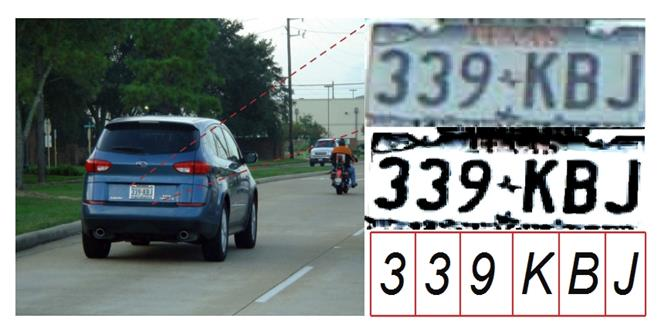
\includegraphics[scale=0.5]{images/carplate}
	\caption{Supaprastinta automobilių numerių atpažinimo schema \cite{PLATEIMG}.}   % Antraštė įterpiama po paveikslėlio
	\label{img:carplate}
\end{figure}
\item Vienas iš seniausių kompiuterinės regos taikymų yra pašto indeksų atpažinimas ant vokų ir siuntinių, leidžiantis sutaupyti daug laiko paštų darbuotojams \cite{POSTCODE}.
\begin{figure}[H]
	\centering
	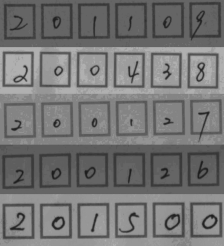
\includegraphics[scale=0.4]{images/postcode}
	\caption{Pašto indeksų pavyzdžiai iš Kinijos pašto.}   % Antraštė įterpiama po paveikslėlio
	\label{img:postcode}
\end{figure}
\item Beveik kiekvieno išmaniojo telefono kameroje yra galimybė naudoti veido aptikimo funkciją.
\item Vietose, kur renkasi dideli pėsčiųjų srautai, skaičiuojamas praeinančių žmonių kiekis. Tam naudojamos įprastos vaizdo kameros vaizdo srautą segmentuojant ir jame išskiriant kiekvieną žmogų atskirai \cite{PEOPLECOUNT}.
\end{itemize}


Darbe yra du skyriai. Literatūros sąraše keturi šaltiniai \cite{BA}.  


\section{ Pirmasis skyrius}
Pirmasis skyrius sudarytas iš dviejų poskyrių. 
\subsection{A1 pavadinimas}
 Tekstas ...
 \subsection{A2 pavadinimas}
 Tekstas su formule $y=x^2$...
 
 %Paveikslas (jpg, png, pdf ir kiti formatai, jei kompiliuojate
 %su pdflatex):
%\[
%\includegraphics[scale=0.8]{mif-logo.png}
%\] 
 
 \section{ Antrasis skyrius}
Antrasis skyrius sudarytas iš trijų poskyrių
\subsection{B1 pavadinimas}
 Tekstas ...
 \subsection{B2 pavadinimas}
 Poskyris B2 turi du skirsnius
 \subsubsection{B21 pavadinimas}
  Tekstas....
  \subsubsection{B22 pavadinimas}
  Tekstas....
 \subsection{B3 pavadinimas}
 Tekstas su nauja formule $y=x^3$...
 
 
\begin{thebibliography}{99}
\addcontentsline{toc}{section}{Literatūra} %% Literatura bus itraukta i turini
\bibitem {OPENCV}
G. Bradski ir A. Kaehler, \textit{Learning OpenCV: Computer vision with the OpenCV library}, O'Reilly Media, Inc., 2008, p. 1–8.

\bibitem {BA}
J. Timothy Smoker, Carrie E. Murphy ir Alison K. Rockwell \textit{Comparing memory for handwriting versus typing}, Proceedings of the Human Factors and Ergonomics Society Annual Meeting. Vol. 53. No. 22. Sage CA: Los Angeles, CA: SAGE Publications, 2009.

\bibitem {CARPLATE}
E. Christos-Nikolaos Anagnostopoulos ir kt., \textit{License plate recognition from still images and video sequences: A survey} IEEE Transactions on intelligent transportation systems 9.3 (2008), p. 377-391.

\bibitem {PRADEEP}
J. Pradeep, E. Srinivasan ir S. Himavathi, \textit{Diagonal based feature extraction for handwritten character recognition system using neural network}, Electronics Computer Technology (ICECT), 2011 3rd International Conference IEEE, 2011.
 
\bibitem {LeCun}
Y. LeCun ir kt., \textit{Comparison of learning algorithms for handwritten digit recognition}, Tarptautinė neuroninių tinklų konferencija, 1995.
\url{http://yann.lecun.com/exdb/publis/pdf/lecun-95b.pdf}

\bibitem{PLATEIMG}
D. Kostadinov, \textit{Privacy Implications of Automatic License Plate Recognition Technology}, \url{http://resources.infosecinstitute.com/privacy-implications-automatic-license-plate-recognition-technology/}.

\bibitem{POSTCODE}
 Shujing Lu ir kt., \textit{Cost-sensitive neural network classifiers for postcode recognition}, International Journal of Pattern Recognition and Artificial Intelligence, 2012.
 
\end{thebibliography} 
 
 
\section*{Santrauka}
\addcontentsline{toc}{section}{Santrauka}
Trumpa darbo santrauka...
\section*{Summary}
\addcontentsline{toc}{section}{Summary}
Short english summary... 



\end{document}
